% Asset ID: AS2StatisticalSamplingTIKZ-003
% Unit: AS2 Applied Mathematics
% Topic: AS2-SAMP Statistical sampling
% Purpose: Stratified sampling proportional allocation
% Source: Supplied Data Collection PDF pages 13-14 and transcript Data Collection 2
% Linked LO IDs: AS2-SAMP-LO003, AS2-SAMP-LO004

\documentclass[tikz,border=8pt]{standalone}
\usetikzlibrary{positioning,arrows.meta,fit}
\begin{document}
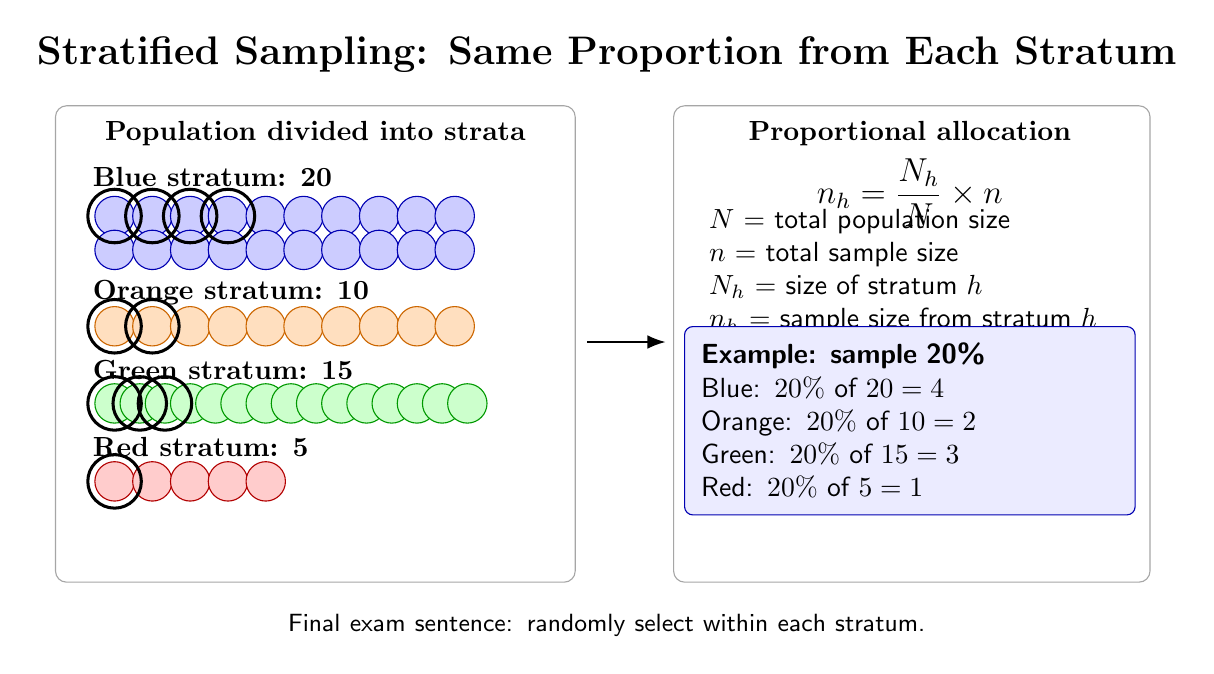
\begin{tikzpicture}[font=\sffamily,arrow/.style={-Latex,thick},panel/.style={draw=black!35,fill=white,rounded corners=4pt,inner sep=8pt}]
\node[font=\bfseries\Large] at (6.4,6.2) {Stratified Sampling: Same Proportion from Each Stratum};
\draw[panel] (-0.6,-0.5) rectangle (6.0,5.55);
\node[font=\bfseries] at (2.7,5.2) {Population divided into strata};
\node[anchor=west,font=\bfseries] at (-0.25,4.65) {Blue stratum: 20};
\node[anchor=west,font=\bfseries] at (-0.25,3.18) {Orange stratum: 10};
\node[anchor=west,font=\bfseries] at (-0.25,2.2) {Green stratum: 15};
\node[anchor=west,font=\bfseries] at (-0.25,1.22) {Red stratum: 5};
\foreach \i in {0,...,9}{\node[circle,draw=blue!70!black,fill=blue!20,minimum size=5mm,inner sep=0pt] at ({0.15+0.48*\i},4.15) {};}
\foreach \i in {0,...,9}{\node[circle,draw=blue!70!black,fill=blue!20,minimum size=5mm,inner sep=0pt] at ({0.15+0.48*\i},3.72) {};}
\foreach \i in {0,1,2,3}{\draw[line width=1.1pt,draw=black] ({0.15+0.48*\i},4.15) circle (3.4mm);}
\foreach \i in {0,...,9}{\node[circle,draw=orange!80!black,fill=orange!25,minimum size=5mm,inner sep=0pt] at ({0.15+0.48*\i},2.75) {};}
\foreach \i in {0,1}{\draw[line width=1.1pt,draw=black] ({0.15+0.48*\i},2.75) circle (3.4mm);}
\foreach \i in {0,...,14}{\node[circle,draw=green!60!black,fill=green!20,minimum size=5mm,inner sep=0pt] at ({0.15+0.32*\i},1.77) {};}
\foreach \i in {0,1,2}{\draw[line width=1.1pt,draw=black] ({0.15+0.32*\i},1.77) circle (3.4mm);}
\foreach \i in {0,...,4}{\node[circle,draw=red!70!black,fill=red!20,minimum size=5mm,inner sep=0pt] at ({0.15+0.48*\i},0.78) {};}
\draw[line width=1.1pt,draw=black] (0.15,0.78) circle (3.4mm);
\draw[arrow] (6.15,2.55) -- (7.15,2.55);
\draw[panel] (7.25,-0.5) rectangle (13.3,5.55);
\node[font=\bfseries] at (10.25,5.2) {Proportional allocation};
\node[font=\bfseries\large] at (10.25,4.45){\(\displaystyle n_h=\frac{N_h}{N}\times n\)};
\node[align=left,text width=5.3cm] at (10.35,3.45){\(N\) = total population size\\ \(n\) = total sample size\\ \(N_h\) = size of stratum \(h\)\\ \(n_h\) = sample size from stratum \(h\)};
\node[draw=blue!70!black,fill=blue!8,rounded corners=3pt,text width=5.3cm,align=left,inner sep=6pt] at (10.25,1.55){\textbf{Example: sample 20\%}\\Blue: \(20\%\) of \(20=4\)\\Orange: \(20\%\) of \(10=2\)\\Green: \(20\%\) of \(15=3\)\\Red: \(20\%\) of \(5=1\)};
\node[align=center,text width=11cm] at (6.4,-1.05){\small Final exam sentence: randomly select within each stratum.};
\end{tikzpicture}
\end{document}
